% !TeX program = xelatex
\documentclass[a4paper,10pt]{article}

% ============================================================================
% កញ្ចប់បណ្ណាល័យ (Packages) – តាមលំនាំ NGS Preah Krasang
% ============================================================================
\usepackage[a4paper, left=0.95cm, right=0.95cm, top=0.85cm, bottom=0.92cm, footskip=0.52cm]{geometry}
\usepackage{amsmath, amssymb}
\usepackage{unicode-math}
\usepackage{fontspec}
\usepackage{array, longtable, colortbl}
\usepackage[table]{xcolor}
\usepackage{pifont}
\usepackage{fancyhdr}
\usepackage{tikz}
\usetikzlibrary{calc, arrows.meta, decorations.pathreplacing, patterns, babel}

% LaTeX 2025 + longtable v4.24 compatibility guard
\makeatletter
\let\@expl@@@mark@update@singlecol@structures@@\relax
\makeatother

% ============================================================================
% ការកំណត់ពុម្ពអក្សរ (Fonts Configuration - Cross-Platform Windows + Cloud fonts/)
% ============================================================================
\providecommand{\NGSFindFonts}{%
  \IfFileExists{C:/Windows/Fonts/cambria.ttc}{%
    \def\NGSSysPath{C:/Windows/Fonts/}%
    \def\NGSUserPath{C:/Users/KIT/AppData/Local/Microsoft/Windows/Fonts/}%
  }{%
    \IfFileExists{./fonts/KhmerOSsiemreap.ttf}{\def\NGSSysPath{./fonts/}\def\NGSUserPath{./fonts/}}{%
    \IfFileExists{../fonts/KhmerOSsiemreap.ttf}{\def\NGSSysPath{../fonts/}\def\NGSUserPath{../fonts/}}{%
    \IfFileExists{../../fonts/KhmerOSsiemreap.ttf}{\def\NGSSysPath{../../fonts/}\def\NGSUserPath{../../fonts/}}{%
    \IfFileExists{../../../fonts/KhmerOSsiemreap.ttf}{\def\NGSSysPath{../../../fonts/}\def\NGSUserPath{../../../fonts/}}{%
    \IfFileExists{../../../../fonts/KhmerOSsiemreap.ttf}{\def\NGSSysPath{../../../../fonts/}\def\NGSUserPath{../../../../fonts/}}{%
    \IfFileExists{../../../../../fonts/KhmerOSsiemreap.ttf}{\def\NGSSysPath{../../../../../fonts/}\def\NGSUserPath{../../../../../fonts/}}{%
    \IfFileExists{../../../../../../fonts/KhmerOSsiemreap.ttf}{\def\NGSSysPath{../../../../../../fonts/}\def\NGSUserPath{../../../../../../fonts/}}{%
      \def\NGSSysPath{../../../../../../../fonts/}\def\NGSUserPath{../../../../../../../fonts/}%
    }}}}}}}%
  }%
}
\NGSFindFonts

\setmathfont[
  Path={\NGSSysPath},
  FontIndex=1,
  Scale=1.02
]{cambria.ttc}

\defaultfontfeatures{Ligatures=TeX}

\setmainfont[
  Path={\NGSUserPath},
  Extension=.ttf,
  Script=Khmer,
  BoldFont={KhmerOSsiemreap},
  BoldFeatures={FakeBold=1.8},
  ItalicFont={KhmerOSsiemreap},
  ItalicFeatures={FakeSlant=0.25},
  BoldItalicFont={KhmerOSsiemreap},
  BoldItalicFeatures={FakeBold=1.8, FakeSlant=0.25}
]{KhmerOSsiemreap}

\newfontfamily\muol[
  Path={\NGSUserPath},
  Extension=.ttf,
  Script=Khmer
]{KhmerOSmuollight}

\newfontfamily\TimesEn[
  Path={\NGSSysPath},
  Extension=.ttf,
  Scale=1.00,
  BoldFont={timesbd},
  ItalicFont={timesi},
  BoldItalicFont={timesbi}
]{times}

\newfontfamily\NagaBold[
  Path={\NGSUserPath},
  Extension=.ttf
]{AKbalthom Naga Bold}

\newfontfamily\CalibriFont[
  Path={\NGSSysPath},
  Extension=.ttf
]{calibri}

\newfontfamily\Tacteing[
  Path={\NGSUserPath}
]{TACTENG.TTF}

\XeTeXlinebreaklocale "km"
\XeTeXlinebreakskip = 0pt plus 1pt minus 0.1pt

% ============================================================================
% ពណ៌ និងទម្រង់ទំព័រ (B&W Print-Safe + Red 5Es Cue)
% ============================================================================
\definecolor{stepgray}{HTML}{D9D9D9}
\definecolor{headgray}{HTML}{F2F2F2}
\definecolor{darkred}{HTML}{C00000}
\definecolor{red5e}{HTML}{FF0000}

\pagestyle{fancy}
\fancyhf{}
\renewcommand{\headrulewidth}{0pt}
\fancyfoot[L]{\fontsize{8.5pt}{10pt}\selectfont អនុវិទ្យាល័យព្រះក្រសាំង --- សេណារីយ៉ូ ២.២ វិធីគុណស្វ័យគុណមាននិទស្សន្តរ៉ឺឡាទីប (\en{EXP\_MUL})}
\fancyfoot[R]{\CalibriFont\fontsize{10.5pt}{12pt}\selectfont\thepage}

\setlength{\parindent}{0pt}
\setlength{\parskip}{0pt}
\setlength{\tabcolsep}{3.5pt}

\newcolumntype{L}[1]{>{\raggedright\arraybackslash}p{#1}}
\newcolumntype{C}[1]{>{\centering\arraybackslash}p{#1}}

% ម៉ាក្រូជំនួយ
\newcommand{\en}[1]{{\TimesEn #1}}
\newcommand{\enbf}[1]{{\TimesEn\textbf{#1}}}
\newcommand{\unit}[1]{\,\text{\en{#1}}}
\newcommand{\fiveE}[1]{{\normalfont\NagaBold\fontsize{9.0pt}{11.5pt}\selectfont\textcolor{red5e}{#1}}}
\newcommand{\timenote}[1]{\textcolor{darkred}{\textit{#1}}}
\newcommand{\cnum}[1]{{\normalfont\fontsize{10.0pt}{12pt}\selectfont\ding{\numexpr181+#1\relax}}\hspace{0.12em}}
\newcommand{\ditem}{\tikz[baseline=-0.5ex]\fill (0,0.42ex) -- (0.42ex,0) -- (0,-0.42ex) -- (-0.42ex,0) -- cycle;\hspace{0.3em}}
\newcommand{\circbox}[1]{\tikz[baseline=(c.base)]\node[draw=black, rounded corners=3pt, line width=0.75pt, inner sep=1.2pt] (c) {\ensuremath{#1}};}
\newcommand{\khmflourish}{{\Tacteing\fontsize{28pt}{11pt}\selectfont\raisebox{-4pt}{3}}}
\newcommand{\secbar}[1]{%
  \par\vspace{5pt}%
  \noindent\colorbox{stepgray}{\makebox[\dimexpr\textwidth-2\fboxsep\relax][l]{\strut\hspace{3pt}{\muol\fontsize{10.5pt}{14pt}\selectfont #1}}}%
  \par\vspace{3pt}%
}
\newcommand{\scenerow}[1]{\multicolumn{4}{|l|}{\cellcolor{headgray}\textbf{#1}} \\* \noalign{\hrule height 0.4pt}}

% ============================================================================
% រូបគំរូក្ដារខៀន និងសញ្ញាណបច្ចេកទេសស-ខ្មៅ (TikZ B&W Quick Reference Panel)
% ============================================================================
\newcommand{\figScenarioRefEXP}{%
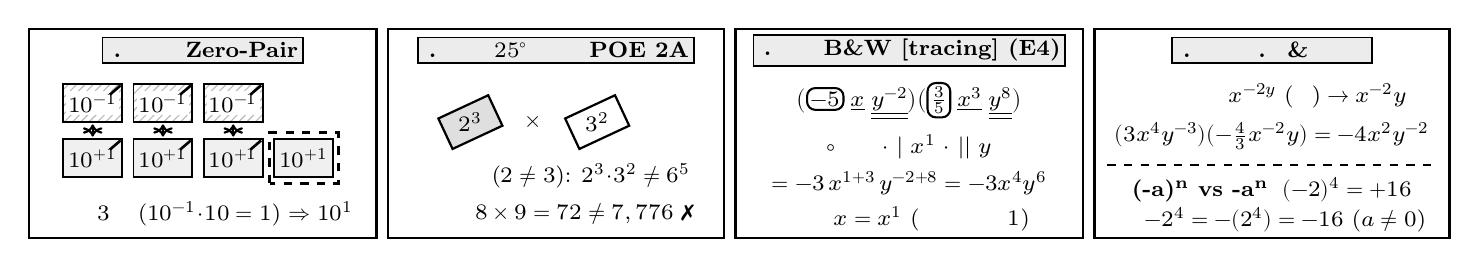
\begin{tikzpicture}[scale=0.97, every node/.style={font=\footnotesize, text=black}]
  % ផ្ទាំង ១៖ ១:១ គូសូន្យ 10^-3 x 10^4
  \draw[black, line width=0.9pt] (0,0) rectangle (4.55,2.74);
  \node[fill=gray!15, draw=black, line width=0.6pt, inner sep=1.8pt] at (2.275,2.46) {\textbf{១. គូសូន្យ \enbf{Zero-Pair}}};
  \foreach \i in {0,1,2} {
    \draw[black, pattern=north east lines, pattern color=gray!55, line width=0.65pt] (0.45+\i*0.92,1.52) rectangle (1.22+\i*0.92,2.02);
    \node[fill=white, inner sep=0.7pt] at (0.835+\i*0.92,1.77) {$10^{-1}$};
  }
  \foreach \i in {0,1,2,3} {
    \draw[black, fill=gray!12, line width=0.65pt] (0.45+\i*0.92,0.80) rectangle (1.22+\i*0.92,1.30);
    \node at (0.835+\i*0.92,1.05) {$10^{+1}$};
  }
  \foreach \i in {0,1,2} {
    \draw[black, densely dashed, line width=0.8pt, <->] (0.835+\i*0.92,1.33) -- (0.835+\i*0.92,1.49);
    \draw[black, line width=0.95pt] (1.06+\i*0.92,1.88) -- (1.20+\i*0.92,2.00);
    \draw[black, line width=0.95pt] (1.06+\i*0.92,1.16) -- (1.20+\i*0.92,1.28);
  }
  \draw[black, line width=1.0pt, dashed] (3.15,0.72) rectangle (4.05,1.38);
  \node at (2.275,0.32) {បន្សាប $3$ គូ ($10^{-1}\!\cdot\!10=1$) $\Rightarrow 10^1$};

  % ផ្ទាំង ២៖ បង្វិល ២៥ ដឺក្រេ អន្ទាក់គោលខុសគ្នា (POE 2A)
  \draw[black, line width=0.9pt] (4.70,0) rectangle (9.10,2.74);
  \node[fill=gray!15, draw=black, line width=0.6pt, inner sep=1.8pt] at (6.90,2.46) {\textbf{២. បង្វិល $25^\circ$ អន្ទាក់ \enbf{POE 2A}}};
  \begin{scope}[shift={(5.78,1.52)}, rotate=25]
    \draw[black, fill=gray!25, line width=0.8pt] (-0.36,-0.22) rectangle (0.36,0.22);
    \node at (0,0) {$2^3$};
  \end{scope}
  \node at (6.60,1.52) {$\times$};
  \begin{scope}[shift={(7.44,1.52)}, rotate=25]
    \draw[black, fill=white, line width=0.8pt] (-0.36,-0.22) rectangle (0.36,0.22);
    \node at (0,0) {$3^2$};
  \end{scope}
  \node at (6.90,0.82) {គោលខុសគ្នា ($2\neq 3$): $2^3\!\cdot\!3^2 \neq 6^5$};
  \node at (6.90,0.32) {តម្លៃពិត $8\times 9=72 \neq 7,776$ \ding{55}};

  % ផ្ទាំង ៣៖ E4 B&W [tracing]
  \draw[black, line width=0.9pt] (9.25,0) rectangle (13.80,2.74);
  \node[fill=gray!15, draw=black, line width=0.6pt, inner sep=1.6pt] at (11.525,2.46) {\textbf{៣. សញ្ញា \enbf{B\&W [tracing]} (\enbf{E4})}};
  \node at (11.525,1.80) {$\bigl(\circbox{-5}\;\underline{x}\;\underline{\underline{y^{-2}}}\bigr)\bigl(\circbox{\tfrac{3}{5}}\;\underline{x^3}\;\underline{\underline{y^8}}\bigr)$};
  \node at (11.525,1.20) {$\circ$ មេគុណ $\cdot$ \textbar{} $x^1$ $\cdot$ \textbar\textbar{} $y$};
  \node at (11.525,0.72) {$= -3\,x^{1+3}\,y^{-2+8} = -3x^4y^6$};
  \node at (11.525,0.26) {\textbf{ចងចាំ៖} $x = x^1$ (និទស្សន្តលាក់ $1$)};

  % ផ្ទាំង ៤៖ Erratum #1 & ដែនវង់ក្រចក
  \draw[black, line width=0.9pt] (13.95,0) rectangle (18.60,2.74);
  \node[fill=gray!15, draw=black, line width=0.6pt, inner sep=1.8pt] at (16.275,2.46) {\textbf{៤. កែពុម្ពទំ.១៥ \& វង់ក្រចក}};
  \node at (16.275,1.86) {\textbf{ប្រតិបត្តិ គ៖} $x^{-2y}\text{ (ខុស)} \to x^{-2}y$};
  \node at (16.275,1.34) {$(3x^4y^{-3})(-\frac{4}{3}x^{-2}y)=-4x^2y^{-2}$};
  \draw[black, line width=0.7pt, dashed] (14.12,0.96) -- (18.43,0.96);
  \node at (16.275,0.64) {\textbf{\enbf{(-a)\textsuperscript{n}} vs \enbf{-a\textsuperscript{n}}៖} $(-2)^4=+16$};
  \node at (16.275,0.24) {រីឯ $-2^4=-(2^4)=-16$ ($a\neq 0$)};
\end{tikzpicture}}

\begin{document}

% ============================================================================
% ក្បាលឯកសារសង្ខេប (Compact Institutional Header)
% ============================================================================
\noindent
\begin{minipage}[t]{0.49\textwidth}
  {\muol\fontsize{10pt}{13.5pt}\selectfont
  មន្ទីរអប់រំ យុវជន និងកីឡា ខេត្តកំពង់ធំ\\
  ការិយាល័យអប់រំ យុវជន និងកីឡា ស្រុកកំពង់ស្វាយ\\
  អនុវិទ្យាល័យព្រះក្រសាំង}
\end{minipage}%
\begin{minipage}[t]{0.50\textwidth}
  \raggedleft
  \textbf{មុខវិជ្ជា៖} គណិតវិទ្យា ថ្នាក់ទី៨ \textbar{} \textbf{រយៈពេល៖} ១ ម៉ោង (៥០ នាទី)\\
  \textbf{កាលបរិច្ឆេទ៖} ៧កើត ខែកត្តិក ឆ្នាំមមី អដ្ឋស័ក ព.ស. ២៥៧០\\
  ត្រូវនឹងថ្ងៃចន្ទ ទី១៦ ខែវិច្ឆិកា ឆ្នាំ២០២៦
\end{minipage}

\vspace{3pt}
\begin{center}
  {\muol\fontsize{12.5pt}{17pt}\selectfont សេណារីយ៉ូបង្រៀនលម្អិត តាមនាទី និងការគ្រប់គ្រងក្ដារខៀន}\\[1pt]
  \khmflourish\\[2pt]
  \textbf{មេរៀនទី២ ស្វ័យគុណ $\cdot$ ២.២. វិធីគុណស្វ័យគុណមាននិទស្សន្តរ៉ឺឡាទីប (ទំ.១៥ និង ២៥)}\\
  \small ក្រុមសិក្សា៖ \textbf{«ក្រុមវិស្វករទិន្នន័យ និងគូសូន្យ ៣ តួនាទី»} $\cdot$ គ្រូបង្រៀន៖ \textbf{ហុក ប៊ុនថែន}
\end{center}
\vspace{3pt}

% ============================================================================
% ផ្នែកទី ១៖ លំហូរសេណារីយ៉ូគ្រប់គ្រងនាទី-ទល់-នាទី (៥០ នាទីសរុប)
% ============================================================================
\secbar{ផ្នែកទី ១៖ លំហូរសេណារីយ៉ូគ្រប់គ្រងនាទី-ទល់-នាទី និងការរៀបចំក្ដារខៀន \enbf{(}២ \enbf{+} ៩ \enbf{+} ១៧ \enbf{+} ២០ \enbf{+} $\le$២ \enbf{=} ៥០ នាទី\enbf{)}}

\fontsize{9.5pt}{13.2pt}\selectfont
\renewcommand{\arraystretch}{1.09}
\begin{longtable}{|L{1.80cm}|L{5.10cm}|L{6.55cm}|L{4.52cm}|}
\hline
\rowcolor{stepgray}
\centering\textbf{នាទី / 5Es} & \centering\textbf{សកម្មភាពគ្រូ និងពាក្យគន្លឹះ} & \centering\textbf{សកម្មភាពសិស្ស និងអន្តរកម្ម} & \centering\textbf{គ្រប់គ្រងក្ដារខៀន \& សម្ភារៈ} \tabularnewline
\hline
\endfirsthead
\hline
\rowcolor{stepgray}
\centering\textbf{នាទី / 5Es} & \centering\textbf{សកម្មភាពគ្រូ និងពាក្យគន្លឹះ} & \centering\textbf{សកម្មភាពសិស្ស និងអន្តរកម្ម} & \centering\textbf{គ្រប់គ្រងក្ដារខៀន \& សម្ភារៈ} \tabularnewline
\hline
\endhead
\hline
\endfoot
\hline
\endlastfoot

% --- ជំហានទី ១ (00-02') ---
\scenerow{ឈុតទី ១ $\cdot$ ជំហានទី១៖ រដ្ឋបាលថ្នាក់ និងបង្កើត «ក្រុមវិស្វករទិន្នន័យ និងគូសូន្យ ៣ តួនាទី» (០០--០២ នាទី | ២ នាទី)}
\textbf{00'--02'}\par\timenote{2 min} &
\ditem ត្រួតពិនិត្យវត្តមាន អនាម័យ សណ្ដាប់ធ្នាប់ថ្នាក់ និងសួរសុខទុក្ខសិស្ស។\par
\ditem ចាត់ក្រុម $3$ នាក់តាមលំដាប់តុ (វេនគ្នា)៖ តួនាទី $1$ កាត់/គូស, $2$ គណនា/ហេតុផល, $3$ ត្រួតសញ្ញា។ &
\ditem ប្រធានថ្នាក់រាយការណ៍វត្តមាន។\par
\ditem ចូលក្រុម ៣ នាក់ស្ងាត់ៗ រៀបចំសៀវភៅ មេរៀនទំ.១៥ និងកន្ត្រៃ/ឈុត \en{P1}។ &
\textbf{ក្ដារឆ្វេង៖} កាលបរិច្ឆេទ + សូចនាករ \en{P1}–\en{P6}។\par
\textbf{តុក្រុម៖} ឈុត \en{P1} ($1$ ឈុត/ក្រុម)។ \\[2pt]
\hline

% --- ជំហានទី ២ ក (02-05') ---
\scenerow{ឈុតទី ២ $\cdot$ ជំហានទី២ ក៖ កំណែ កិច្ចការផ្ទះមេរៀន ២.១ (០២--០៥ នាទី | $\le$៣ នាទី)}
\textbf{02'--05'}\par\timenote{$\le$3 min} &
\ditem ហៅសិស្ស $2$ នាក់សរសេរចម្លើយ \textbf{២.១}៖ ទំ.១៤ \textbf{ប្រតិបត្តិ ២ គ.} និងទំ.២៥ \en{\#1} ខ.។\par
\ditem ជួយស្ទង់ចំណុចខុស (-៨) មានវង់ក្រចក និងគ្មានវង់ក្រចក ($n$ សេស/គូ)។ &
\ditem ឡើងសរសេរ៖ $(-2)^7=-128$ និង $(-8)\cdots(-8)=(-8)^6$ ($6$ កត្តា)។\par
\ditem កត់ត្រាវិន័យវង់ក្រចក $(-8)^6 \neq -8^6$ ចូលសៀវភៅ។ &
\textbf{ក្ដារឆ្វេង៖} កំណែ ២.១\par
$(-2)^7=-128$; $(-8)^6$ ($6$ កត្តា)។\par
សង្កត់៖ $(-8)^6 \neq -8^6$។ \\[2pt]
\hline

% --- ជំហានទី ២ ខ (05-08') ---
\scenerow{ឈុតទី ៣ $\cdot$ ជំហានទី២ ខ៖ រំលឹកស្ពានចំណេះដឹង ២.១ ភ្ជាប់និទស្សន្ត ០ និងអវិជ្ជមាន (០៥--០៨ នាទី | ៣ នាទី)}
\textbf{05'--08'}\par\timenote{3 min} &
\ditem បង្ហាញលំនាំចែក $10$ ចុះពី $10^2$ ដល់ $10^{-3}$ និងបញ្ជាក់លក្ខខណ្ឌ $a\neq 0$។\par
\ditem រំលឹករហ័សបូកចំនួនគត់៖ $-3+4$, $-2+8$, $-3+1$ ដើម្បីត្រៀមបូកនិទស្សន្ត។ &
\ditem ឆ្លើយផ្ទាល់មាត់៖ $10^2=100 \to 10^1=10 \to 10^0=1 \to 10^{-1}=\frac{1}{10}$ និង $10^{-3}=\frac{1}{10^3}$។\par
\ditem គណនារហ័ស៖ $-3+4=1$, $-2+8=6$, $-3+1=-2$។ &
\textbf{ក្ដារឆ្វេង៖} តារាងចែក $10$ និងច្បាប់ $a^0=1, a^{-n}=\frac{1}{a^n}$ ($a\neq 0$)។\par
បូកចំនួនគត់៖ $1, 6, -2$។ \\[2pt]
\hline

% --- ជំហានទី ២ គ E1 (08-11') ---
\scenerow{ឈុតទី ៤ $\cdot$ ជំហានទី២ គ / \fiveE{E1 Engage}៖ បេសកកម្មឃ្លាំងវីដេអូ Server បណ្ណាល័យឌីជីថលព្រះក្រសាំង (០៨--១១ នាទី | ៣ នាទី)}
\textbf{08'--11'}\par\fiveE{E1 Engage}\par\timenote{3 min} &
\ditem ប្រកាសបេសកកម្ម \en{Server} បណ្ណាល័យឌីជីថលអនុវិទ្យាល័យព្រះក្រសាំង៖ ថត $2^3$ មាន $2^4$ វីដេអូ និងឯកសារបង្ហាប់ $10^{-3}\unit{MB}\times 10^4$។\par
\ditem បោះជម្រើស \en{POE} $3$ គំនិត៖ $2^7$, $4^7$, ឬ $2^{12}$? ទាយមុនដោយគ្មានការវិនិច្ឆ័យ។ &
\ditem លើកដៃបោះឆ្នោតទស្សន៍ទាយមុន (\en{P1})៖ តើ $2^3\times 2^4$ ស្មើ $2^7$, $4^7$ ឬ $2^{12}$? តើ $10^{-3}\times 10^4$ កើន ឬថយ? &
\textbf{ក្ដារកណ្ដាល (កំពូល)៖} ចំណងជើងមេរៀន \textbf{២.២} + សំណួរ \en{E1} បើកចំហ ($2^3\times 2^4=?$, $10^{-3}\times 10^4=?$)។ \\[2pt]
\hline

% --- ជំហានទី ៣ ក E2 (11-22') ---
\scenerow{ឈុតទី ៥ $\cdot$ ជំហានទី៣ ក / \fiveE{E2 Explore}៖ ពិសោធន៍ ១:១ បន្ទះកត្តា កម្រាលគូសូន្យ និងអន្ទាក់ POE 2A–2B (១១--២២ នាទី | ១១ នាទី)}
\textbf{11'--14'}\par\fiveE{E2 Act 1a}\par\timenote{3 min} &
\ditem \textbf{សកម្មភាព ១ក (\en{P1 1:1})៖} ផ្ទៀងខ្នាត $5.00\unit{cm}$។ តម្រៀបបន្ទះ $2^3$ ($3.00\unit{cm}$) តនឹង $2^4$ ($4.00\unit{cm}$)។ &
\ditem វាស់សរុបបាន $7.00\unit{cm} \Rightarrow 2^7$ កត្តា; កំណត់៖ មិនគុណគោល $2\times 2$ ជា $4$ ទេ! &
\textbf{តុក្រុម (\en{P1})៖} បន្ទះ $1:1$\par
$3+4=7 \to 2^7$។ \\[2pt]

\textbf{14'--17'}\par\fiveE{E2 Act 1b}\par\timenote{3 min} &
\ditem \textbf{សកម្មភាព ១ខ (\en{Zero-Pair})៖} ដាក់កាតឆ្នូត $3$ បន្ទះ ($10^{-1}$) ទល់នឹងកាតរាប $4$ បន្ទះ ($10^{+1}$) រួចគូស \en{/}។ &
\ditem គូសខ្វែង $3$ គូ ($10^{-1}\cdot 10 = 1$) នៅសល់កាតរាប $1$ បន្ទះ $= 10^1 = 10$។ &
\textbf{ក្ដារកណ្ដាល៖} កម្រាលគូសូន្យ $-3+4=1 \to 10^1$។ \\[2pt]

\textbf{17'--19.5'}\par\fiveE{E2 Act 2a}\par\timenote{2.5 min} &
\ditem \textbf{សកម្មភាព ២ក (\en{POE 2A})៖} បង្ហាញប្លុកបង្វិល $25^\circ$ ($2^3\times 3^2$)៖ តើ $2^3\cdot 3^2 = 6^5$ ឬ $2^3\cdot 2^4 = 4^7$? &
\ditem គណនាតម្លៃពិត៖ $8\times 9 = 72 \neq 6^5$; $8\times 16=128\neq 4^7$។ \textbf{គោលខុសគ្នា ហាមបូកនិទស្សន្ត}។ &
\textbf{ក្ដារកណ្ដាល (\en{POE 2A})៖}\par
$2^3\cdot 3^2\neq 6^5$; $2^3\cdot 2^4\neq 4^7$។ \\[2pt]

\textbf{19.5'--22'}\par\fiveE{E2 Act 2b}\par\timenote{2.5 min} &
\ditem \textbf{សកម្មភាព ២ខ (\en{POE 2B})៖} បោះអន្ទាក់ $3^2\cdot 3^3 \stackrel{?}{=} 3^6$ (គុណនិទស្សន្ត!) និង $a\cdot a^3 \stackrel{?}{=} a^3$ (ភ្លេច $a=a^1$)។ &
\ditem កែអន្ទាក់ \en{2B}៖ $3^2\cdot 3^3 = 3^{2+3}=3^5\neq 3^6$ និង $a^1\cdot a^3 = a^{1+3}=a^4$។ &
\textbf{ក្ដារកណ្ដាល (\en{POE 2B})៖}\par
$3^2\cdot 3^3\neq 3^6$; $a=a^1$។ \\[2pt]
\hline

% --- ជំហានទី ៣ ខ E3 (22-28') ---
\scenerow{ឈុតទី ៦ $\cdot$ ជំហានទី៣ ខ / \fiveE{E3 Explain}៖ សិស្សបង្គុំទ្រឹស្ដីបទ កែ Erratum \#2 និងធនាគារហេតុផល \cnum{1}–\cnum{5} (២២--២៨ នាទី | ៦ នាទី)}
\textbf{22'--28'}\par\fiveE{E3 Explain}\par\timenote{6 min} &
\ditem ឱ្យសិស្សសង្ខេបរូបមន្តជាភាសាខ្លួនឯងមុន ទើបបើកទំ.១៥ \textbf{ឧទាហរណ៍ ក–ឃ} និង \textbf{ជាទូទៅ}។\par
\ditem សង្កត់ \textbf{\en{Erratum \#2}}៖ $a\neq 0$ បើ $m\le 0$ ឬ $n\le 0$ (ឧ. $a^2\cdot a^{-2}=a^0=1$) និងបិទផ្ទាំង \en{P4} \cnum{1}–\cnum{5}។ &
\ditem បង្កើតតារាង សម្មតិកម្ម--សន្និដ្ឋាន--វិបាក ($a^m\cdot a^n = a^{m+n}$, $a\neq 0$)។\par
\ditem ប្រើលេខហេតុផល \cnum{1} គោលដូចគ្នា, \cnum{2} បូកនិទស្សន្ត, \cnum{3} $x=x^1$, \cnum{4} ផ្ដុំមេគុណ, \cnum{5} $a^{-n}=1/a^n$។ &
\textbf{ក្ដារកណ្ដាល (បំពេញរូបមន្ត)៖}\par
$a^m\cdot a^n=a^{m+n}$ ($a\neq 0$ បើ $m,n\le 0$)។\par
\textbf{ជញ្ជាំងថ្នាក់៖} បិទផ្ទាំង \en{P4} \cnum{1}–\cnum{5}។ \\[2pt]
\hline

% --- ជំហានទី ៤ ក E4 (28-38') ---
\scenerow{ឈុតទី ៧ $\cdot$ ជំហានទី៤ ក / \fiveE{E4 Elaborate}៖ លំហាត់គំរូ ក–គ (ទំ.១៥) សញ្ញា B\&W [tracing] \& CE-EE (២៨--៣៨ នាទី | ១០ នាទី)}
\textbf{28'--38'}\par\fiveE{E4 Elaborate}\par\timenote{10 min} &
\ditem ចែកកាត \en{P2} បង្រៀនស៊ើបអង្កេត $3$ ជំហាន៖ ព័ទ្ធរង្វង់មេគុណ, គូស \textbar{} ក្រោម $x$, \textbar\textbar{} ក្រោម $y$, ធ្នូបូកនិទស្សន្ត។\par
\ditem អនុវត្តលំហាត់គំរូ \textbf{ក.} $10^{-3}\times 10^4$, \textbf{ខ.} $(-5y^2)(7y^8)$ (គ្រូដឹកនាំ) និង \textbf{គ.} $(-5xy^{-2})(\frac{3}{5}x^3y^8)$ (សិស្សបញ្ចប់ + \en{EIA Looking-Back})។ &
\ditem គូស \en{[tracing]} លើកាត \en{P2} ព្រមគ្នា៖ រកឃើញ $x = x^1$, បំបែកលេខ $-5\times \frac{3}{5}=-3$, ស្វ័យគុណ $x^{1+3}=x^4$, $y^{-2+8}=y^6$។\par
\ditem ពិនិត្យត្រឡប់ (\en{EIA})៖ ហេតុអ្វីមិនទទួល $-3x^3y^6$? (ព្រោះ $x=x^1$!)។ &
\textbf{ក្ដារស្ដាំ៖} បង្ហាញកាត \en{P2} ៣ ជំហាន + \en{[tracing]}\par
គំរូ ក $=10$; ខ $=-35y^{10}$; គ $=-3x^4y^6$។ \\[2pt]
\hline

% --- ជំហានទី ៤ ខ E5 & ជំហានទី ៥ (38-50') ---
\scenerow{ឈុតទី ៨ $\cdot$ ជំហានទី៤ ខ (\fiveE{E5 Evaluate}: ១០') \& ជំហានទី៥ (កិច្ចការផ្ទះ: $\le$២') (៣៨--៥០ នាទី | ១២ នាទី)}
\textbf{38'--43'}\par\fiveE{E5 Relay}\par\timenote{5 min} &
\ditem \textbf{\en{Relay P3} (ប្រតិបត្តិ ក–គ ទំ.១៥)៖} បញ្ឈប់សួរ \en{Pause-Ask!} មុនប្តូរវេន និង \en{Pause-Review!} មុនផ្ទៀងផ្លូវការ។\par
\ditem ប្រកាស \textbf{\en{Erratum \#1}}៖ កែ $x^{-2y}\to x^{-2}y$ ក្នុង \textbf{គ.} រួចបិទបញ្ចប់បេសកកម្ម \en{E1}។ &
\ditem តួនាទី $1$ គូស \en{[tracing]}, $2$ គណនា + \cnum{1}–\cnum{5}, $3$ ផ្ទៀងសញ្ញាដក៖\par
ក. $x^{13}$, ខ. $1$, គ. $-4x^2y^{-2}$។\par
\ditem សរុប \en{E1}៖ $2^7=128$ វីដេអូ; $10\unit{MB}$។ &
\textbf{ក្ដារស្ដាំ៖} ចម្លើយ \en{Relay P3}\par
ក. $x^{13}$; ខ. $(-\frac{3}{2})^0=1$; គ. $-4x^2y^{-2}$ (កែពុម្ព)។ \\[3pt]

\textbf{43'--48'}\par\fiveE{E5 Exit}\par\timenote{5 min} &
\ditem ចែកកាត \en{P5} វិនិច្ឆ័យគំរូ \en{A–D} (សិស្សលើកសញ្ញា \ding{51}/\ding{55}) រួចធ្វើ \en{Exit Ticket} ៣ សំណួរដោយឯករាជ្យ ($2.5$ នាទី)។ &
\ditem វិនិច្ឆ័យ \en{B} ត្រូវ, \en{A, C, D} ខុស (គុណគោល / គុណនិទស្សន្ត / វង់ក្រចក $-2^4$)។\par
\ditem ឆ្លើយ \en{Exit}៖ $5^4$; $-8x^{-2}y^2$; គោល $2\neq 3$។ &
\textbf{តុសិស្ស (\en{P5})៖} ប័ណ្ណឆ្លើយ \en{A–D} + \en{Exit Ticket} ($1–3$) ប្រមូលមុខចេញ។ \\[3pt]

\textbf{48'--50'}\par\textbf{ជំហានទី៥}\par\timenote{$\le$2 min} &
\ditem កាត់ចែកប័ណ្ណ \en{P6}៖ ផ្នែក ក ទំ.២៥ \en{\#6} ក, ខ, គ (ប្រយ័ត្ន $2=2^1$) និងផ្នែក ខ \en{\#7} ខ (ជៀសវាង \en{\#7} ក ខុសពុម្ព) + ស្ពាន ២.៣។ &
\ditem ទទួលប័ណ្ណ \en{P6} និងគិតទុកសំណួរស្ពាន ២.៣៖ ហេតុអ្វី $2^7\cdot 2^{-4}$ ដូច $\frac{2^7}{2^4}$? &
\textbf{ក្ដារស្ដាំ (បាត)៖} លេខលំហាត់ផ្ទះទំ.២៥៖ \en{\#6} ក–គ, \en{\#7} ខ + អានមុនទំ.១៦។ \\[2pt]
\end{longtable}

% ============================================================================
% ផ្នែកទី ២៖ បញ្ជីសម្ភារៈស-ខ្មៅ (P1-P6) និងផ្ទាំងគំរូក្ដារខៀន
% ============================================================================
\secbar{ផ្នែកទី ២៖ បញ្ជីសម្ភារៈបោះពុម្ពស\enbf{-}ខ្មៅ \enbf{(P1–P6)} និងផ្ទាំងគំរូបច្ចេកទេសសំខាន់ៗ}

\fontsize{9.5pt}{13.1pt}\selectfont
\renewcommand{\arraystretch}{1.09}
\begin{longtable}{|C{1.15cm}|L{6.00cm}|L{10.95cm}|}
\hline
\rowcolor{headgray}
\textbf{ទំព័រ} & \textbf{ឈ្មោះសម្ភារៈ (ពី Printable Materials)} & \textbf{គោលបំណង និងការប្រើប្រាស់ស-ខ្មៅ (B\&W Print-Safe)} \tabularnewline
\hline
\endfirsthead
\hline
\rowcolor{headgray}
\textbf{ទំព័រ} & \textbf{ឈ្មោះសម្ភារៈ (ពី Printable Materials)} & \textbf{គោលបំណង និងការប្រើប្រាស់ស-ខ្មៅ (B\&W Print-Safe)} \tabularnewline
\hline
\endhead
\hline
\endfoot
\hline
\endlastfoot
\textbf{\en{P1}} & បន្ទះកត្តា ១:១, កម្រាលគូសូន្យ \& តារាង \en{POE 2A–2B} & ខ្នាតផ្ទៀង $5.00\unit{cm}$ (\en{Actual Size 100\%})៖ កាត់បន្ទះ $2^3, 2^4$ តម្រៀប $7.00\unit{cm}$ និងគូស \en{/} លើគូសូន្យ $10^{-3}\times 10^4$ ($1$ ឈុត/ក្រុម)។ \\
\hline
\textbf{\en{P2}} & កាតស៊ើបអង្កេត $3$ ជំហាន \& សញ្ញា \en{[tracing]} ($E4$) & បោះ $2\text{-up}$ លើកំណត់ \textbf{លំហាត់គំរូ ក–គ} ទំ.១៥ ដោយគូសរង្វង់មេគុណ, \textbar{} ក្រោម $x$, \textbar\textbar{} ក្រោម $y$, និងធ្នូបូកនិទស្សន្ត។ \\
\hline
\textbf{\en{P3}} & សន្លឹក \en{Relay} ៣ តួនាទី ($E5$) & បោះ $2\text{-up}$ លើ \textbf{ប្រតិបត្តិ ក–គ} ទំ.១៥ (កែ \en{Erratum \#1} $x^{-2y}\to x^{-2}y$) + \en{Pause-Ask!} \& \en{Pause-Review!} + បិទបញ្ចប់បេសកកម្ម \en{E1}។ \\
\hline
\textbf{\en{P4}} & ផ្ទាំងប្រកាសថ្នាក់ (\en{Warrant Bank} \cnum{1}–\cnum{5}) & បិទមុខថ្នាក់៖ \textbf{ជាទូទៅ} (\en{Erratum \#2} $a\neq 0$), ដែនវង់ក្រចក $(-a)^n$ vs $-a^n$, ហេតុផល \cnum{1}–\cnum{5} និងស្ពានមេរៀន ២.៣។ \\
\hline
\textbf{\en{P5}} & កាតវិនិច្ឆ័យ \en{A–D} \& ប័ណ្ណ \en{Exit Ticket} & \en{A–D} ($B$ ត្រូវ, $A,C,D$ ខុស) សម្រាប់បង្ហាញភ្លាម + សំណួរ $3$ ធាតុ ($\le 90$ វិនាទី) វាយតម្លៃមុនចប់ម៉ោង។ \\
\hline
\textbf{\en{P6}} & ប័ណ្ណកិច្ចការផ្ទះ ៤-ក្នុង-១ (ផ្នែក ក \& ខ) & ផ្នែក ក (\en{\#6} ក–គ ទំ.២៥) និងផ្នែក ខ (\en{\#7} ខ ទំ.២៥, ជៀសវាង \en{\#7} ក ខុសពុម្ព) + សំណួរស្ពាន $2^7\cdot 2^{-4}$ vs $\frac{2^7}{2^4}$។ \\
\end{longtable}

\vspace{4pt}
\noindent\figScenarioRefEXP

% ============================================================================
% ផ្នែកទី ៣៖ តារាងការយល់ច្រឡំតាមឯកសារស្រាវជ្រាវ និងវិធានការទប់ស្កាត់
% ============================================================================
\secbar{ផ្នែកទី ៣៖ តារាងការយល់ច្រឡំ និងការការពារកំហុសផ្អែកលើភស្តុតាងស្រាវជ្រាវ \enbf{(Evidence 01–15)}}

\fontsize{9.5pt}{13.2pt}\selectfont
\renewcommand{\arraystretch}{1.10}
\begin{longtable}{|L{3.50cm}|L{4.25cm}|L{5.10cm}|L{5.10cm}|}
\hline
\rowcolor{headgray}
\textbf{ប្រភេទកំហុសជាញឹកញាប់} & \textbf{ភស្តុតាងអត្រាខុសជាក់ស្ដែង} & \textbf{មូលហេតុគរុកោសល្យ / ការយល់ច្រឡំ} & \textbf{វិធានការបង្ការក្នុងម៉ោងនេះ (5Es)} \tabularnewline
\hline
\endfirsthead
\hline
\rowcolor{headgray}
\textbf{ប្រភេទកំហុសជាញឹកញាប់} & \textbf{ភស្តុតាងអត្រាខុសជាក់ស្ដែង} & \textbf{មូលហេតុគរុកោសល្យ / ការយល់ច្រឡំ} & \textbf{វិធានការបង្ការក្នុងម៉ោងនេះ (5Es)} \tabularnewline
\hline
\endhead
\hline
\endfoot
\hline
\endlastfoot
\textbf{១. គុណគោលដូចគ្នា ឬខុសគ្នា}\par ($2^3\!\cdot\!2^4=4^7$; $2^3\!\cdot\!3^2=6^5$) & \en{Ulusoy (2019)} (\en{N=165}): \en{Q7} ខុស $61.8\%$ ($16.9\%$ គុណគោល); \en{Pournara \& Bowie (2023)} (\en{N=589}): $36.2\%$ សរសេរ $6^5$។ & ជួសជុលខុសតាមការគុណលេខធម្មតា ដោយបង្កើតគោលថ្មី $a\cdot a$ ឬ $a\cdot b$ ហើយបូកនិទស្សន្ត។ & បន្ទះ $1:1$ \en{P1} (\en{E2 Act 1}) រក្សាគោលថេរ + អន្ទាក់ \en{POE 2A} ប្លុកបង្វិល $25^\circ$ និងច្រក \cnum{1}។ \\
\hline
\textbf{២. គុណនិទស្សន្តជំនួសឱ្យការបូក}\par ($3^2\cdot 3^3=3^6$; $a\cdot a^4\cdot a^{-2}=a^{-8}$) & \en{Ulusoy (2019)}: \en{Q6} $5^{-2}\cdot 5^4$ ខុស $59.4\%$ ($8.4\%$ គុណនិទស្សន្ត); \en{Pournara \& Bowie (2023)}: $\sim 60\%$ ថ្នាក់ទី៨ ច្រឡំច្បាប់។ & លាយឡំសញ្ញា «គុណស្វ័យគុណ» ជាមួយការយកនិទស្សន្តមកគុណគ្នា ($2\times 3$) ឬច្រឡំមេរៀន ២.៤។ & អន្ទាក់ \en{POE 2B} (\en{E2}), និទស្សន្តកាត \en{P5 Exit Foil C}, និងលុបគូសូន្យ $10^{-3}\times 10^4$។ \\
\hline
\textbf{៣. ភ្លេចនិទស្សន្តលាក់ $1$ និងផ្ដុំអញ្ញាត}\par ($a\cdot a^3=a^3$; $x\cdot x^3=x^3$) & \en{Pournara et al. (2016)} (\en{N=250}): $47\%\text{–}59\%$ ផ្តោតលើលេខមុនអក្សរ, $42\%\text{–}53\%$ បញ្ចូលអញ្ញាតខុស។ & មើលមិនឃើញលេខ $1$ លើ $x, y, 2$ និងច្រឡំអក្សរខុសគោលពេលគុណឯកធាមានច្រើនអញ្ញាត។ & សញ្ញា \en{B\&W [tracing]} (\en{E4}, \en{Yeo \& Tzeng 2019, p=.003}): រង្វង់មេគុណ, \textbar{} $x$, \textbar\textbar{} $y$, និង \cnum{3} $x=x^1$។ \\
\hline
\textbf{៤. វង់ក្រចក និងសញ្ញាដកមុខគោល}\par ($(-2)^4=-16$; $(-3)^0$ vs $-3^0$) & \en{Olson et al. (2011)}: $5/19$ ត្រូវ ($6/19$ ថាវង់ក្រចកមិនសំខាន់); \en{Ulusoy (2019)}: \en{Q1} ខុស $66.1\%$; \en{Aydın-Güç (2021)}: $50\%$ បោះសញ្ញាដក។ & មិនញែកវង់ក្រចក $( -a )^n$ ពី $-a^n$ និងបោះសញ្ញាដកមុខឯកធាចោលពេលគុណលេខអវិជ្ជមាន។ & កំណែ ២.១, តួនាទីទី $3$ ត្រួតសញ្ញា \en{Pause-Review!} (\en{P3}), ផ្ទាំងដែនវង់ក្រចក \en{P4}, និង \en{Foil D}។ \\
\hline
\textbf{៥. កំហុសពុម្ពសៀវភៅសិក្សា និងដែន $a\neq 0$}\par (ទំ.១៥ \textbf{ប្រតិបត្តិ គ.}, \textbf{ជាទូទៅ}) & សៀវភៅក្រសួងទំ.១៥ បោះពុម្ព $x^{-2y}$ (ខុស), ទំ.២៥ \en{\#7} ក. ខ្វះកត្តា, និងខ្វះ $a\neq 0$ ក្នុង \textbf{ជាទូទៅ}។ & ការទុកបណ្ដោយកំហុសពុម្ពនាំឱ្យសិស្សបូកនិទស្សន្តលេខជាមួយអក្សរ ឬចែកនឹង $0$។ & កែ \textbf{\en{Erratum \#1}} ($x^{-2}y$), \textbf{\en{Erratum \#2}} ($a\neq 0$), ជ្រើស \en{\#7} ខ ជំនួស \en{\#7} ក, និងបង្រួម \en{E1–E5} គ្រប់ $50$ នាទី។ \\
\hline
\end{longtable}

\end{document}
